%!TEX root = ../doc.tex
\chapter{Implementierung MoveIt! Package}\label{sec:ImplementierungMontage}
Im folgenden Kapitel wird anhand des Stäubli Roboters TX2-60l erläutert, wie das MoveIt! Package für ROS-I erzeugt wird. Dieses Vorgehen wurde mit leichten Abänderungen auch auf den IRB120 von ABB und den UR3 von Universal Robots angewendet. Es ist wäre auch möglich andere Roboter so in den Industrie Demonstrator einzubinden.\\

Zur Erzeugung des MoveIt! Packages wird ein .xacro File benötigt. Für den IRB120 und UR3 sind diese Pakete bereits im ROS-I Gitrepository vorhanden, wobei das Package für den IRB120 unter dem Status experimentell aufgeführt wird. Die für den Stäubliroboter generierten Files werden im Ordner /staubli\_expermiental/staubli\_tx260l\_support abgelegt. Für den Stäubli Roboter musste ein Package aufgesetzt werden. Dazu wurden folgende Schritte durchgeführt:
\begin{enumerate}
	\item Erstellen Visual- und Kollisionsmodelle
	\item Erstellen .xacro File
	\item Generieren MoveIt! Package
	\item Anpassungen für ROS-I
\end{enumerate}

\section{Erstellen Visual- und Kollisionsmodelle}
\subsection{Roboter und Greifer}
Die CAD-Modelle des TX2-60l wurden von der Website von Stäubli bezogen, anschliessend musste an den Modellen gemäss den ROS/ROS-I Konventionen einige Anpassungen gemacht werden. Diese beinhalten vor allem Anpassungen am Koordinatensystem. Die ROS-Konventionen bestimmen, dass relativ zu den Körpern die x-Achse nach vorne Zeigt, die y-Achse nach links und die z-Achse nach oben.\\
Damit an Rechenleistung gespart werden kann, werden für die Kollisionsberechnung vereinfachte CAD-Modelle verwendet. Diese wurden mithilfe der Software Meshlab, welche gratis verfügbar ist, erstellt. Meshlab bietet diverse Tools und Funktionen um .stl-Files, sowie auch andere Tesselationsfiles zu bearbeiten. Für die Kollisionsfiles werden die CAD-Files mithilfe des Tools 'Convex Hull' vereinfacht (Vergleich Abbildung \ref{fig:Collision} und \ref{fig:visual}). Die erstellten Modelle werden in den entsprechenden Unterordnern abgelegt.\\

\begin{figure} []
	\begin{minipage}[h]{0,49\textwidth}
		\centering
			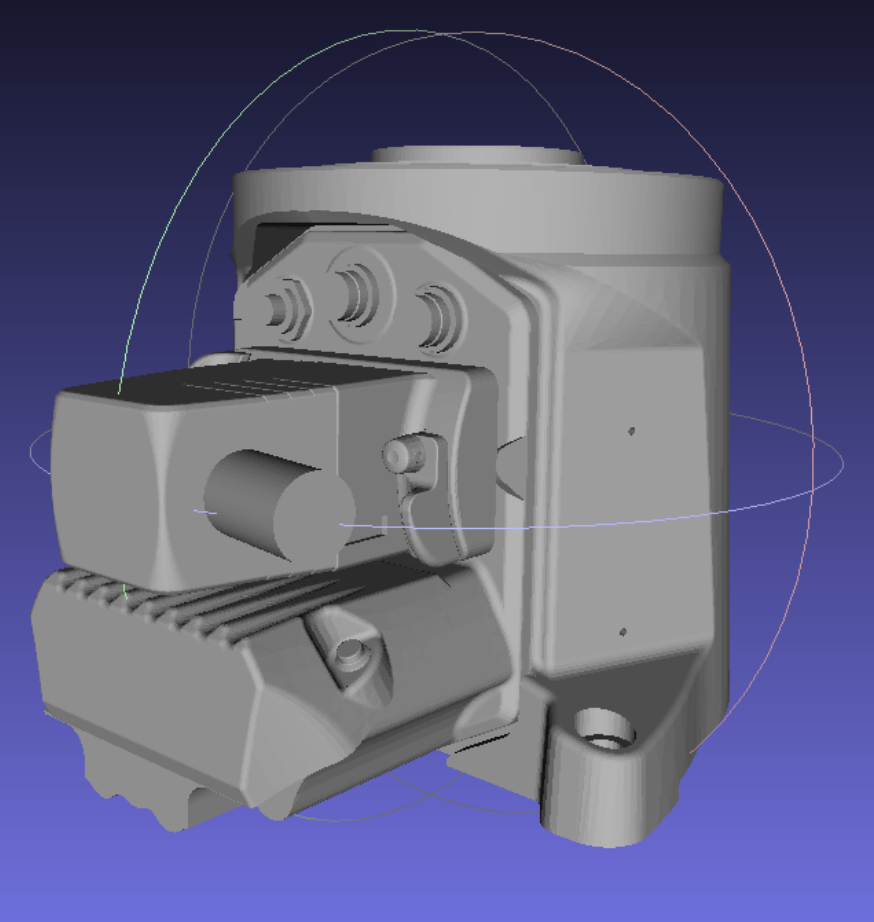
\includegraphics[width=0.95\textwidth]{visual}
		\caption{Visuelles Modell der Base TX2-60l}
		\label{fig:visual}
	\end{minipage}
	\begin{minipage}[h]{0,49\textwidth}
		\centering
			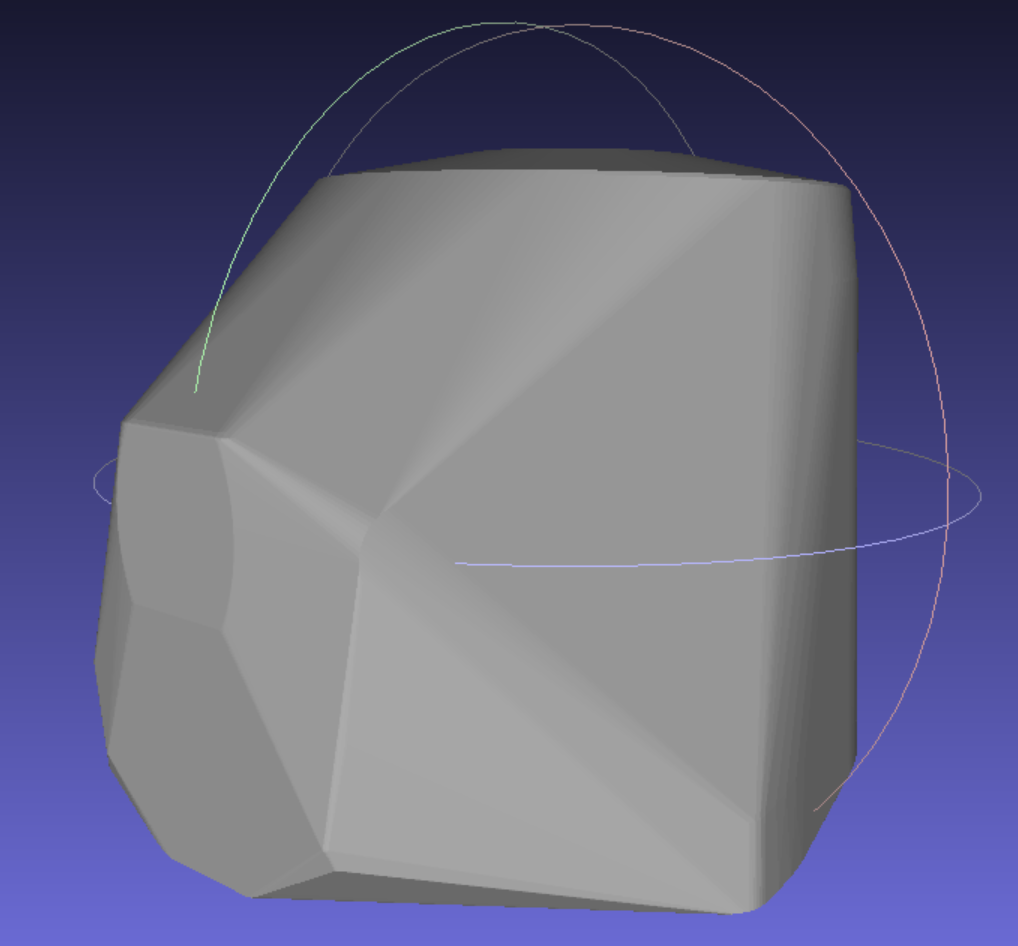
\includegraphics[width=0.95\textwidth]{collision}
		\caption{Kollisions Modell der Base TX2-60l}
		\label{fig:Collision}
	\end{minipage}
\end{figure}
Das selbe Vorgehen wurde auch für den Greifer durchgeführt, bei diesem wurde die Convex Hull jedoch nur auf den hinteren Teil des Greifers angewendet.  

\subsection{Anlage}
Aufgrund der Grösse und Komplexität der Anlage ist auch das CAD-Modell sehr gross. MoveIt! hat starke Schwierigkeiten sehr grosse Files zu laden, aus diesem  Grund wurde der visuelle Teil der Anlage mithilfe von Meshlab stark vereinfacht. Somit konnte die Dateigrösse von 240MB auf circa 50MB verringert werden, diese Grösse lässt sich einigermassen gut importieren und visualisieren.\\
Für das Kollisionsmodell wurde nur der mittlere Teil der Anlage verwendet und stark vereinfacht. Ein Grossteil wird dabei einfach als Box dargestellt (siehe Abbildung \ref{fig:collisionAnlage}).

\begin{figure} [H]
	\begin{minipage}[h]{0,49\textwidth}
		\centering
		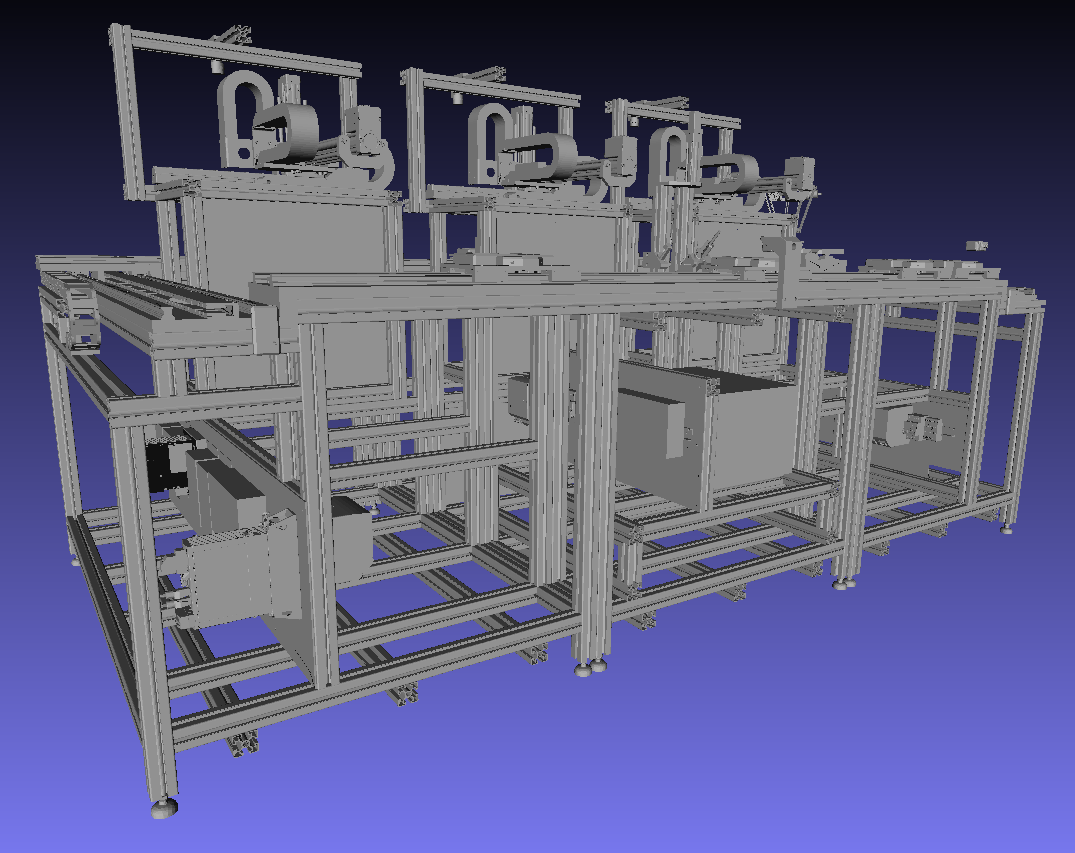
\includegraphics[width=0.95\textwidth]{visualAnlage}
		\caption{Visuelles Modell}
		\label{fig:visualAnlage}
	\end{minipage}
	\begin{minipage}[h]{0,49\textwidth}
		\centering
		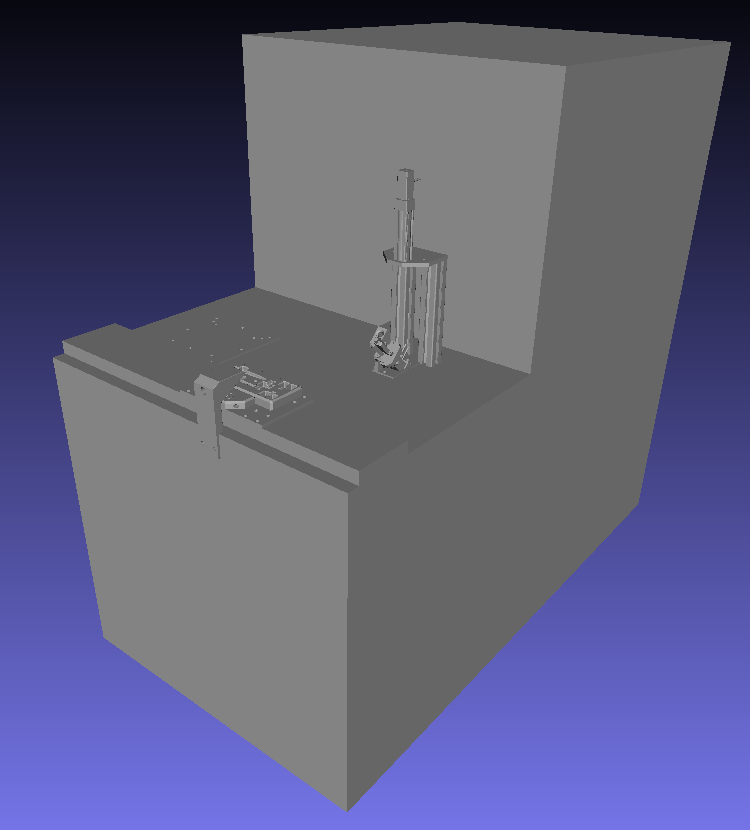
\includegraphics[width=0.95\textwidth]{collisionAnlage}
		\caption{Kollisions Modell}
		\label{fig:collisionAnlage}
	\end{minipage}
\end{figure}

\section{xacro Files}
Für die Einbindung des Roboters in die Montageanlage wurden vier unterschiedliche xacro-Files erstellt. Das erste beschreibt den Roboter, das zweite den Greifer und das dritte beschreibt die Anlage. Diese drei Files werden in einem übergeordneten File, welches die ganze Anlage beschreibt eingebunden. Dies ermöglicht es den Roboter in der Montagezelle einfach auszuwechseln. 
\subsection{Roboter}
Zur Beschreibung des Roboters wird ein xacro-macro File erstellt, die dafür benötigten Masse werden aus dem Datenblatt des TX2-60l bezogen. Für die Massenträgheitsmomente der einzelnen Glieder konnten keine Angaben gefunden werden. Auch für den maximalen Kraftaufwand (Effort) eines Gelenkes wurden keine Angaben Gefunden. Aus diesem Grund wurden die selben Werte wie die des Vorgängermodells TX-60l verwendet, da dieser in etwa die gleichen Abmessungen wie sein Nachfolger besitzt. Falls die Bewegungsabläufe mit dem echten Roboter nicht Konform sind müssen allenfalls diese Werte angepasst werden. Im folgenden wird je ein Beispiel für ein Gelenk und ein Glied des Roboters gezeigt, das komplette File ist im Anhang unter \ref{Anhang:Staublixacro} zu finden.

\begin{code}
	\begin{minted}{xml}
<link name="${prefix}base_link">
	<visual>
		<origin xyz="0 0 0" rpy="0 0 0" />
		<geometry>
			<mesh filename="package://staubli_tx260l_support/meshes/tx260l/visual/base_link.stl" />
		</geometry>
		<xacro:material_staubli_ral_melon_yellow />
	</visual>
	<collision>
		<origin xyz="0 0 0" rpy="0 0 0" />
		<geometry>
			<mesh filename="package://staubli_tx260l_support/meshes/tx260l/collision/base_link.stl" />
		</geometry>
	</collision>
	<inertial>
		<mass value="5.76415" />
		<origin xyz="-0.010284 -0.000676 0.087340" rpy="0.0 0.0 0.0" />
		<inertia ixx="0.000025" ixy="-0.000001" ixz="-0.000002" iyy="0.000034" iyz="-0.0000001" izz="0.000029" />
	</inertial>
</link>
	\end{minted}
	\vspace{-15pt}
	\caption{Definition des Baselinks TX2-60l}
	\label{code:baseLink}
\end{code}
\begin{code}
	\begin{minted}{xml}
<joint name="${prefix}joint_2" type="revolute">
	<origin xyz="0.0 0.130 0.375" rpy="0 0 0" />
	<parent link="${prefix}link_1" />
	<child link="${prefix}link_2" />
	<axis xyz="0 1 0" />
	<limit lower="-2.22529" upper="2.22529" effort="130.0" velocity="6.719" />
	<dynamics damping="0.0" friction="0.0" />
</joint>
	\end{minted}
	\vspace{-15pt}
	\caption{Definition der zweiten Achse TX2-60l}
	\label{code:joint}
\end{code}

Anschliessend muss ein neues File generiert werden, welches das vollständig definierte tx260l\_macro.xacro einschliesst. Damit aus diesem ein URDF mithilfe der folgenden Kommandozeileneingabe erstellt werden kann.
\begin{code}
	\begin{minted}{bash}
rosrun xacro xacro.py tx260l.xacro > tx260l_generated.urdf	
	\end{minted}
	\vspace{-15pt}
	\caption{Generierung des URDF aus xacro}
	\label{code:xacroToURDF}
\end{code}
Schlussendlich müssen sich im Unterordner folgende drei Files befinden.
\dirtree{%
	.1 urdf .
	.2 tx260l\_generated.urdf .
	.2 tx260l\_macro.xacro .
	.2 tx260l.xacro .
}

\subsection{Greifer}
Der Greifer besteht, wie auch der Roboter, aus einem Visuellen und einem Kollisionsmodell. Zudem besitzt der Greifer zwei unterschiedliche Greiferframes auf welche die move\_group planen kann, somit ist es möglich den Greifer richtig zu Positionieren um die Teile zu greifen. Die Positionen der beiden Frames wurden in der Abbildung \ref{fig:Greifer} in Form zweier Kugeln visualisiert.
\begin{figure}[H]
	\centering
	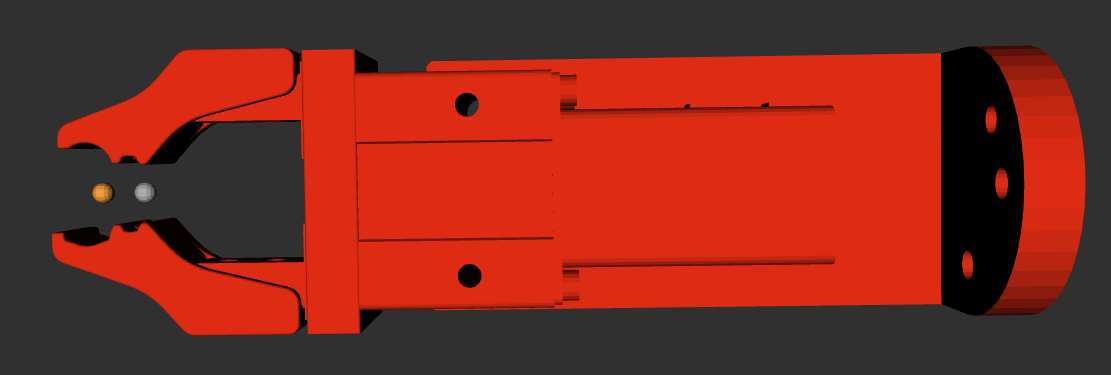
\includegraphics[width=0.8\textwidth]{greifer}
	\caption{Visualisierung der Greiferframes}
	\label{fig:Greifer}
\end{figure}

\subsection{Unterbau}
Im xacro der Anlage wird nur das Visuelle Modell der Anlage geladen, da ansonsten die Ladezeiten beim starten der move\_group extrem hoch sind und diese oft abstürzt. Das Kollisionsobjekt wird sobald die move\_group gestartet ist eingebunden (siehe Abschnitt \ref{sec:penAssembly}). Falls bei einem xacro kein Kollisionsobjekt definiert wird, wird automatisch der visuelle Teil auch für die Kollisionsberechnung verwendet. Aus diesem Grund wurde als Kollisionsobjekt eine Kugel mit Radius $0.1\;mm$ definiert und so positioniert, das diese sich in der Base des Roboters befindet.
\begin{code}
	\begin{minted}{xml}
<collision>
	<origin rpy="0 0 0" xyz="0 0 0.005" />
	<geometry>
		<sphere radius="0.0001" />
	</geometry>
</collision>	
	\end{minted}
	\vspace{-15pt}
	\caption{Dummy Kollisionsobjekt der Anlage}
	\label{code:dummyAnlage}
\end{code}

\subsection{Gesammte Anlage}
Die generierten Einzelteile der Anlage werden anschliessend in einem einzelnen .xacro-File eingebunden, als Ankerpunkt für den Greifer, Roboter und den Unterbau wird ein leerer Link mit dem Namen World definiert.
\begin{code}
	\begin{minted}{xml}
<?xml version="1.0" ?>
	<robot name="cell_tx260l" xmlns:xacro="https://ros.org/wiki/xacro">
	<xacro:include filename="$(find cell_support)/urdf/gripper_definition.xacro"/>
	<xacro:include filename="$(find cell_support)/urdf/unterbau.xacro" />
	<xacro:include filename="$(find staubli_tx260l_support)/urdf/tx260l_macro.xacro"/>
	
	<link name="world"/>
	
	<!-- init robots -->
	<xacro:gripper_definition prefix="" />
	<xacro:unterbau prefix=""/>
	<xacro:staubli_tx260l prefix="" />
	
	<!-- Joints -->
	<joint name="world_to_tx260l" type="fixed">
		<parent link="world" />
		<child link="base_link"/>
		<origin xyz="0 0 0" rpy="0 0 0"/>
	</joint>  
	<joint name="world_to_unterbau" type="fixed">
		<parent link="world" />
		<child link="unterbau_base"/>
		<origin xyz="0 0 0" rpy="0 0 0"/>
	</joint> 
	<joint name="tool0_to_gripper" type="fixed">
		<parent link="tool0" />
		<child link="gripper_base" />
		<origin xyz="0 0 0" rpy="0 1.57 0" />
	</joint>
</robot>	
	\end{minted}
	\vspace{-10pt}
	\caption{.xacro-File der gesammten Anlage}
	\label{code:xacroAnlage}
\end{code}

\section{MoveIt! Konfiguration}\label{sec:MoveitSetup}
Das erstellen der MoveIt! Konfiguration muss für alle Roboter welche in der Anlage eingebaut werden sollen durchgeführt werden, die Einstellungen sind dabei für alle Roboter identisch. Nachfolgend sind alle vorgenommenen Einstellungen aufgelistet, welche im Setup Assistant vorgenommen wurden.\\
\paragraph{Self-Collisions}
Als erstes wird der Setup Assistant gestartet und das .xacro-File geladen, anschliessend kann im Tab Self-Collisions die Kollisionsmatrix erstellt. Dabei kann die Sampling Density auf High gestellt werden.
\paragraph{Virtual Joints} Als nächstes muss ein Virtual Joint definiert werden, dieses verbindet die simulierte Welt mit dem geladenen .xacro-File, als Child Link wird dabei der definierte Ankerlink World gewählt, das Parent Frame ist World, und der Joint Type ist fixed. Als Name wurde hier jeweils FixedBase gewählt, dieser kann jedoch frei gewählt werden.
\paragraph{Planning Groups}
Es müssen zwei Planungsgruppen erstellt werden, eine small\_gripper und eine gripper. Je eine für die unterschiedlichen Frames des Greifers. Beide Planungsgruppen werden als Kinematische Kette definiert mit Start beim base\_link des Roboters und als Ende das entsprechende Frame. Als Kinematischersolver kann aus drei Standard Solvern gewählt werden und dem zusätzlich installierten Solver von TRACLabs. Für alle Roboter und Kinematischen Ketten wird der Solver 'trac\_ik\_kinematics' von TracLab gewählt. Es hat sich in Tests gezeigt, dass der Solver von TRACLabs, im Vergleich zu den Standardsolvern, fast immer eine Lösung findet. Die Einstellungswerte des Solvers wurde dabei auf den Standartwerten belassen.
\paragraph{Robot Poses}
Im Tab Robot Poses können Positionen des Roboters definiert werden, welche im \gls{GUI} der move\_group direkt ausgewählt werden können. Hier wurden zwei Posen definiert, eine mit allen Gelenken in Nullposition und eine Warteposition. 
\paragraph{End Effectors}
Im Abschnitt End Effectors muss nichts eingestellt werden. Hier würden Endeffektoren, die von der move\_group gesteuert werden definiert werden.
\paragraph{Passive Joints}
Im Abschnitt Passive Joints muss nichts angepasst werden. Hier würden Gelenke definiert werden, welche nicht angetrieben sind.
\paragraph{Author Information}
Es müssen Namen und Emailadressen des Erstellers diese Packages angegeben werden, ansonsten lässt sich das Setup nicht beenden.
\paragraph{Configuration Files}
In diesem Setup muss der Pfad angegeben werden, wo das Package abgespeichert werden soll, der Paketname muss, gemäss den ROS-Konventionen, dabei auf

'\_moveit\_config' enden. % das muss so sein!!


\section{Anpassungen ROS-I}
Für ROS-Industrial müssen nach dem Erstellen des Packages mit dem Setup Assistant einige Dateien hinzugefügt, respektive abgeändert werden. 
\paragraph{controllers.yaml}
Als erstes muss die Datei 'controllers.yaml' im config Ordner erzeugt werden, welche den ROS-Node 'Controller Manager' zur Verfügung stellt der von der move\_group gebraucht wird. Die Datei ist für alle Roboter gleich. Es muss jedoch beachtet werden, dass die Bezeichnungen der Gelenke mit deren des Roboters übereinstimmen müssen. 
\begin{code}
	\begin{minted}{yaml}
controller_list:
      - name: ""
      action_ns: joint_trajectory_action
      type: FollowJointTrajectory
      joints: [joint_1, joint_2, joint_3, joint_4, joint_5, joint_6]
	\end{minted}
	\vspace{-15pt}
	\caption{controller.yaml}
	\label{code:controller}
\end{code}

\paragraph{controller\_manager.launch}
Das .launch-File um den Controller zu starten ist nach dem Erstellen der Konfiguration zwar vorhanden jedoch ist es leer. Das File muss für jeden Roboter spezifisch angepasst werden. Es benötigt den Pfad zum jeweiligen 'controller.yaml'. Nachfolgend eine Vorlage, bei welcher der Teil in den eckigen Klammern ergänzt werden muss.
\begin{code}
	\begin{minted}{xml}
<launch>
	<arg name="moveit_controller_manager"
	  default="moveit_simple_controller_manager/MoveItSimpleControllerManager"/>
	<param name="moveit_controller_manager"
	      value="$(arg moveit_controller_manager)"/>	
	<rosparam file="$(find [robot_moveit_config])/config/controllers.yaml"/>
</launch>	
	\end{minted}
	\vspace{-15pt}
	\caption{Vorlage '..controller\_manager.launch'}
	\label{code:controllerManager}
\end{code}

\paragraph{moveit\_planning\_execution.launch}
Als letztes muss ein .launch-File erzeugt werden, welches alle für ROS-I benötigten Nodes startet. Eine Vorlage dieses Files ist im Anhang unter \ref{Anhang:MoveitVorlage} zu finden. Auch in diesem File müssen einige Teile spezifisch auf die Roboter angepasst werden. 
\section{ROS}
Damit ROS-I mit dem Roboter Kommunizieren kann muss auf den Robotersteuerungen Anpassungen vorgenommen werden.
\paragraph{ABB IRB 120}
Für den ABB IRB120 ist es nötig einen ROS Server auf dem Controller des Roboters zu installieren. Es müssen einige neue Tasks auf der Steuerung erstellt werden sowie ein RAPID-Programm auf die Steuerung geladen werden. Eine sehr detaillierte Anleitung dazu ist auf den ROS-Wikipages\footnote{\url{http://wiki.ros.org/abb/Tutorials/InstallServer}} zu finden.

\paragraph{Stäubli TX2-60l}
Da der Stäubli Roboter bei Abschluss dieser Arbeit noch nicht geliefert wurde können keine konkreten Angaben über die nötigen Anpassungen auf dem Controllers gemacht werden. Es stehen Driver für die Steuerung CS8 zur Verfügung, gemäss Informationen von Stäubli wird der Roboter mit einer Steuerung vom Typ CS9 geliefert. Bei Erhalt des Roboters und der Steuerung müssen diese mit ROS getestet werden und allenfalls der Server für die Steuerung angepasst werden. Die benötigten Files sowie eine Anleitung in Form eines Readmes befinden sich im Ordner /staubli\_expermintal/staubli\_val3\_driver.

\paragraph{Universal UR3}
Für den Universal Robot UR3 muss keine zusätzliche Software installiert werden, da Universal Robot Standardmässig auf ihrer Steuerung bereits ROS Messages verarbeiten kann. Somit genügt es auf der Robotersteuerung das Netzwerk zu konfigurieren respektive kontrollieren ob dieses eingeschaltet ist. 